\documentclass[b5paper,12pt]{jsreport}
\usepackage[top=2cm,bottom=2cm,left=2.5cm,right=2.5cm]{geometry}

\usepackage{bm}
% \usepackage[dvipdfmx]{graphicx}
\usepackage{ascmac}

% 画像読み込みよう
\usepackage[dvipdfmx]{graphicx}

\usepackage{caption}

\usepackage{color}
\newcommand{\red}[1]{\textcolor{red}{#1}}

\usepackage{booktabs}
\usepackage{adjustbox}

\usepackage{url}


% \usepackage[dvipdfmx]{graphicx}
% \usepackage[dvipdfmx]{color}

\setlength{\parskip}{2mm} % 3mmのスペースを挿入

% インデントを無効化
\setlength{\parindent}{0pt}


\title{多言語自動翻訳掲示板の利活用に関する実践研究}
\author{早稲田大学人間科学部人間情報科学科\\
西村研究室\\
\\
学籍番号:1J20F037\\
名前:奥村飛悠}

\date{\today}
\renewcommand{\bibname}{参考引用文献}
\begin{document}
\maketitle
\tableofcontents

\chapter{はじめに}

\section{現状}

インターネットの普及やソーシャルメディアの台頭により,オンラインでのコミュニケーションが一般的になっている(大向,2006).その中でも,誰でも気軽に参加することのできる掲示板は重要なコミュニケーションの場となっている.日本では,"5ちゃんねる"(サイト名を"2ちゃんねる"から"5ちゃんねる"へ2017年10月に変更)が広く知られている一方で,米国発の"reddit"は国際的に認知度が高く,日別のアクティブユーザー数は5700万人,総投稿数は130億投稿を超えている(Reddit Inc,2023).これらの大規模な掲示板は情報の集積場所として,またユーザー間の活発な議論の場として重要な役割を果たしている.

しかしながら,掲示板は誰もが利用できるコミュニケーションの場であるにも関わらず,現状ではそのコミュニケーションは主に同一言語間で行われている.具体的には,"5ちゃんねる"では主に日本語,"reddit"では主に英語が使用されている.そのため,異なる言語を使用するユーザーは,翻訳ツールや外部の翻訳サービスを頼るか,専用のスレッドや言語コミュニティを探すことが一般的となっている.しかし,これらの方法にはデメリットが存在する.例えば,翻訳ツールを利用すると時間と手間がかかるため,掲示板の持つ即時性や気軽さというメリットを十分に享受することが難しくなる.

同一言語間でのコミュニケーションが主流となっている背後には複数の要因が考えられるが,その一つとして翻訳技術の品質が十分でなかったことが考えられる.2004年には「コミュニケーションツールとして使用する場合に十分な品質を持っているとはいい難い」(船越ほか,2004)との指摘があり,さらに2010年にも「近年,翻訳技術は急速に進展しているが,高精度な翻訳を行うことは困難である.コミュニケーションにおいて,不適切な翻訳箇所を含む文章は話者間の相互理解を困難にし,円滑なコミュニケーションの妨げとなる」(宮部ほか,2010)とも指摘されている.また,多言語間でのコミュニケーションにおいては,翻訳の品質が極めて大きな影響力を持つことも確認されている(船越ほか,2004).このように,コミュニケーションに大きな影響を与える翻訳技術の品質が十分でなかったため,ユーザーは翻訳技術を利用して会話の中心となっている言語以外を使用してまで会話を試みなかったのではないだろうか.

\section{翻訳技術の進歩}

しかしながら,翻訳サービスの精度は日々向上している.これについて,「近年,Google翻訳やDeepL,そしてページ全体翻訳機能の進化が著しい」(村本,2022)との報告があり,その背景には機械学習の進歩が影響を与えている.「Google英日翻訳がNMT(ニューラル機械翻訳)を採用したことで,目標言語の流暢さが格段に向上した」(影浦,2017)との報告がある.同様にNMTを採用しているDeepLは,2017年にサービスを開始し,その高品質な翻訳サービスが評価されている(亀田,2022).さらに「2020年と2021年には,文章の意味をより正確に伝えられ,業界特有の専門用語もうまく処理できる新たなモデルを発表」(DeepL,2023)している.これらのことから,翻訳サービスの精度は日々向上されていることが分かる.

また,多くの翻訳サービスが開発者向けにAPIを提供している.その代表例としては,Google CloudのTranslation AI(Google Cloud,2023)やDeepL API(DeepL,2023)がある.これらのサービスを開発者が利用するための便利なライブラリも存在している.具体的には,Google Translate API(現在のTranslation AI)を利用するためのPythonのライブラリであるgoogletrans(PyPI,2023a)やdeepl(PyPI,2023b)がある.このようなAPIやライブラリの存在により,開発者は翻訳機能を自身のサービスに容易に組み込むことが可能となっている.

\section{既存サービスと先行研究}

過去には,"enjoy Korea"という日本語と韓国語の翻訳機能を持つ掲示板サービスが存在していたが,利用率の低下を理由に2009年6月8日にサービスを終了している(野津,2009).また,小川ら(2009)は日本語とウイグル語間の翻訳掲示板システムを開発している.しかし,彼らの研究は主にシステムの開発に焦点を当てており,システムを使用するユーザーのデータ収集やその分析までには至っていない.

一方,藤井ら(2005)はアノテーションや折り返し翻訳に着目し,中国語,韓国語,日本語間の翻訳BBSである"AnnoChat"を開発した.翻訳の精度がコミュニケーションの理解度に影響を与える可能性を示しているが,ユーザー同士の具体的なコミュニケーションの内容までは調査していない.また,吉野ら(2006)はユーザインタフェースのカスタマイズ性に焦点を当てた研究を行い,"CustomChat"というシステムを開発したが,これも具体的なチャットの内容などについては触れられていない.

これらの事例や研究を見ると,多言語間のコミュニケーションを可能にする翻訳掲示板に関する研究やサービスは確かに存在している.しかし,それらは主にシステムの開発や翻訳の精度と理解度の関係性,ユーザインタフェースの改良に焦点を当てており,異なる言語を使用するユーザーがシステムをどのように使うのか,どのようなコミュニケーションが起こるのかという点については,まだ十分に研究されていないと言える.

\section{本研究の概要と目的}

これらの背景から,本研究では,掲示板のグローバル化を進めるため,近年の高精度な翻訳サービスを利用した多言語自動翻訳掲示板の開発とその利活用について実践的な研究を行う.我々が提案する多言語自動翻訳掲示板では,ユーザーは表示言語を選択することにより,選択した言語で掲示板の投稿を閲覧することを可能にする機能をつける.これにより,異なる言語を使用するユーザー間でも,自由なコミュニケーションが促進され,掲示板の持つ即時性や気軽さというメリットを維持することができる.

そして,この掲示板をインターネット上に公開し,使用者から得られるデータを収集する.その後,得られたデータを分析し,多言語自動翻訳掲示板がユーザーのコミュニケーションにどのような影響を与えるのか,多言語自動翻訳掲示板上で異なる言語を使用するユーザー同士がどのようなコミュニケーションをするのかを評価する.具体的には,ユーザー間のコミュニケーション量や内容,トピックの多様性,言語間のコミュニケーション方法などを指標として用いる.

我々の研究は,新たな掲示板の形を示すだけでなく,機械翻訳技術とその実用化の進歩に貢献することを期待している.本研究の結果が,ユーザーが自由に多言語コミュニケーションを享受できるインターネットの環境整備に向けた一歩となることを願っている.

\chapter{多言語自動翻訳掲示板について}

\section{システムの概要}

本研究では,多言語自動翻訳掲示板である「The Channel」というWebアプリケーションを開発した.このシステムは,世界中のユーザーが自分の言語で投稿することができる.そして,その投稿はユーザーが選択した言語に翻訳されて表示されることで,ユーザーは好きな言語でコンテンツを読むことができる.

システムの中核は,機械翻訳技術が担っている.これにより,ユーザーが投稿したテキストはリアルタイムで他の言語に翻訳され,多様なユーザーがアクセスできるようになる.例えば,日本語で書かれた投稿は,英語,スペイン語,中国語などに瞬時に翻訳され,異なる言語のユーザー間の交流を可能にする.

システムは,掲示板として必要最低限の機能を備えている.ユーザーは簡単にスレッドを作成することや,自分の母国語でコメントを投稿することができる.

セキュリティに考慮し,ユーザーの個人名やメールアドレス等を取り扱わないようにしている.

\section{主な機能と利用フロー}

掲示板は以下の機能を持つ.
\begin{enumerate}
	\item スレッド作成
	
	スレッドの作成を行う.
	\item コメント投稿
	
	スレッドに対して,コメントを投稿する.
	\item 閲覧
	
	スレッドに投稿されたコメントの閲覧.
	\item 言語選択
	
	閲覧する言語を選択する.
\end{enumerate}

以下にシステム利用フローを示す.

\begin{figure}[htbp]
	\centering
	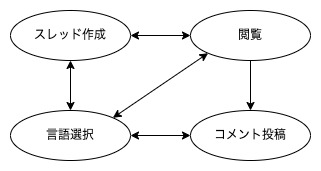
\includegraphics[width=90mm,height=45mm]{img/system.jpg}

	\caption{システム利用フロー}
\end{figure}

\begin{enumerate}
	\item ユーザーはスレッド一覧やスレッドに投稿されたコメントを閲覧することができる.
	\item ユーザーは閲覧しているスレッドに対してコメントを投稿することができる.
	\item ユーザーは自由にスレッドを作成することができる.
	\item ユーザーはいつでも言語を選択することができる.
\end{enumerate}


\section{機能詳細と主な画面操作}

主な画面のフローを以下に示す.

\begin{figure}[htbp]
	\centering
	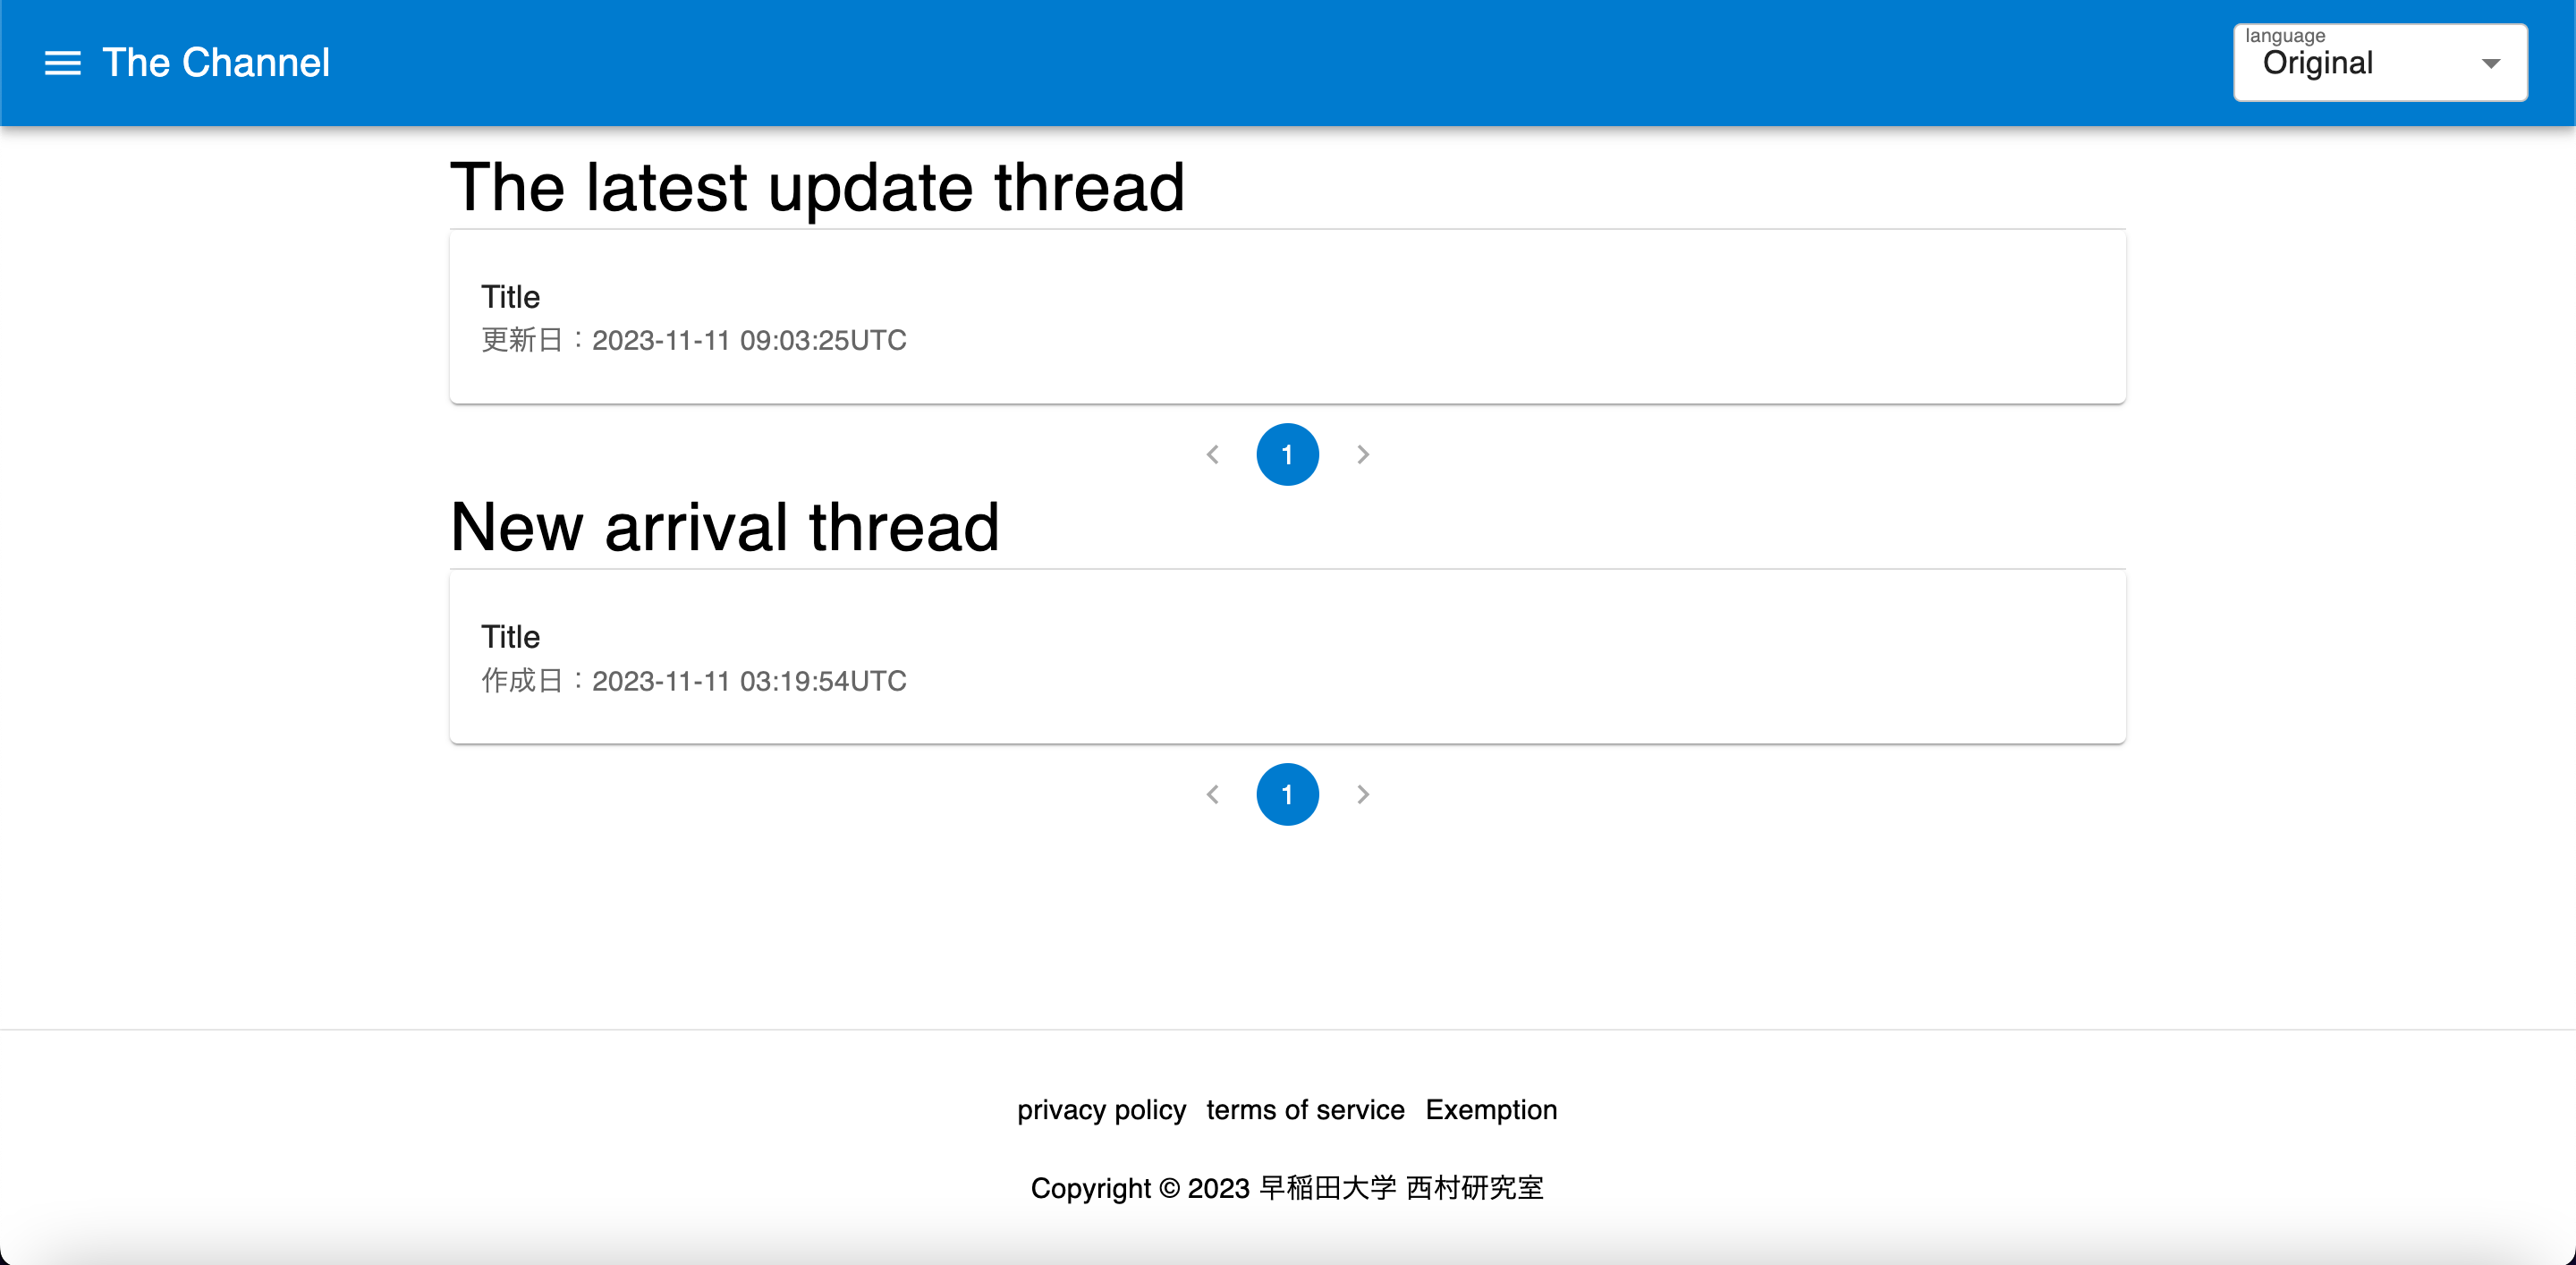
\includegraphics[width=90mm,height=45mm]{img/home.png}

	\caption*{①トップページ画面}
\end{figure}
\begin{figure}[htbp]
	\centering
	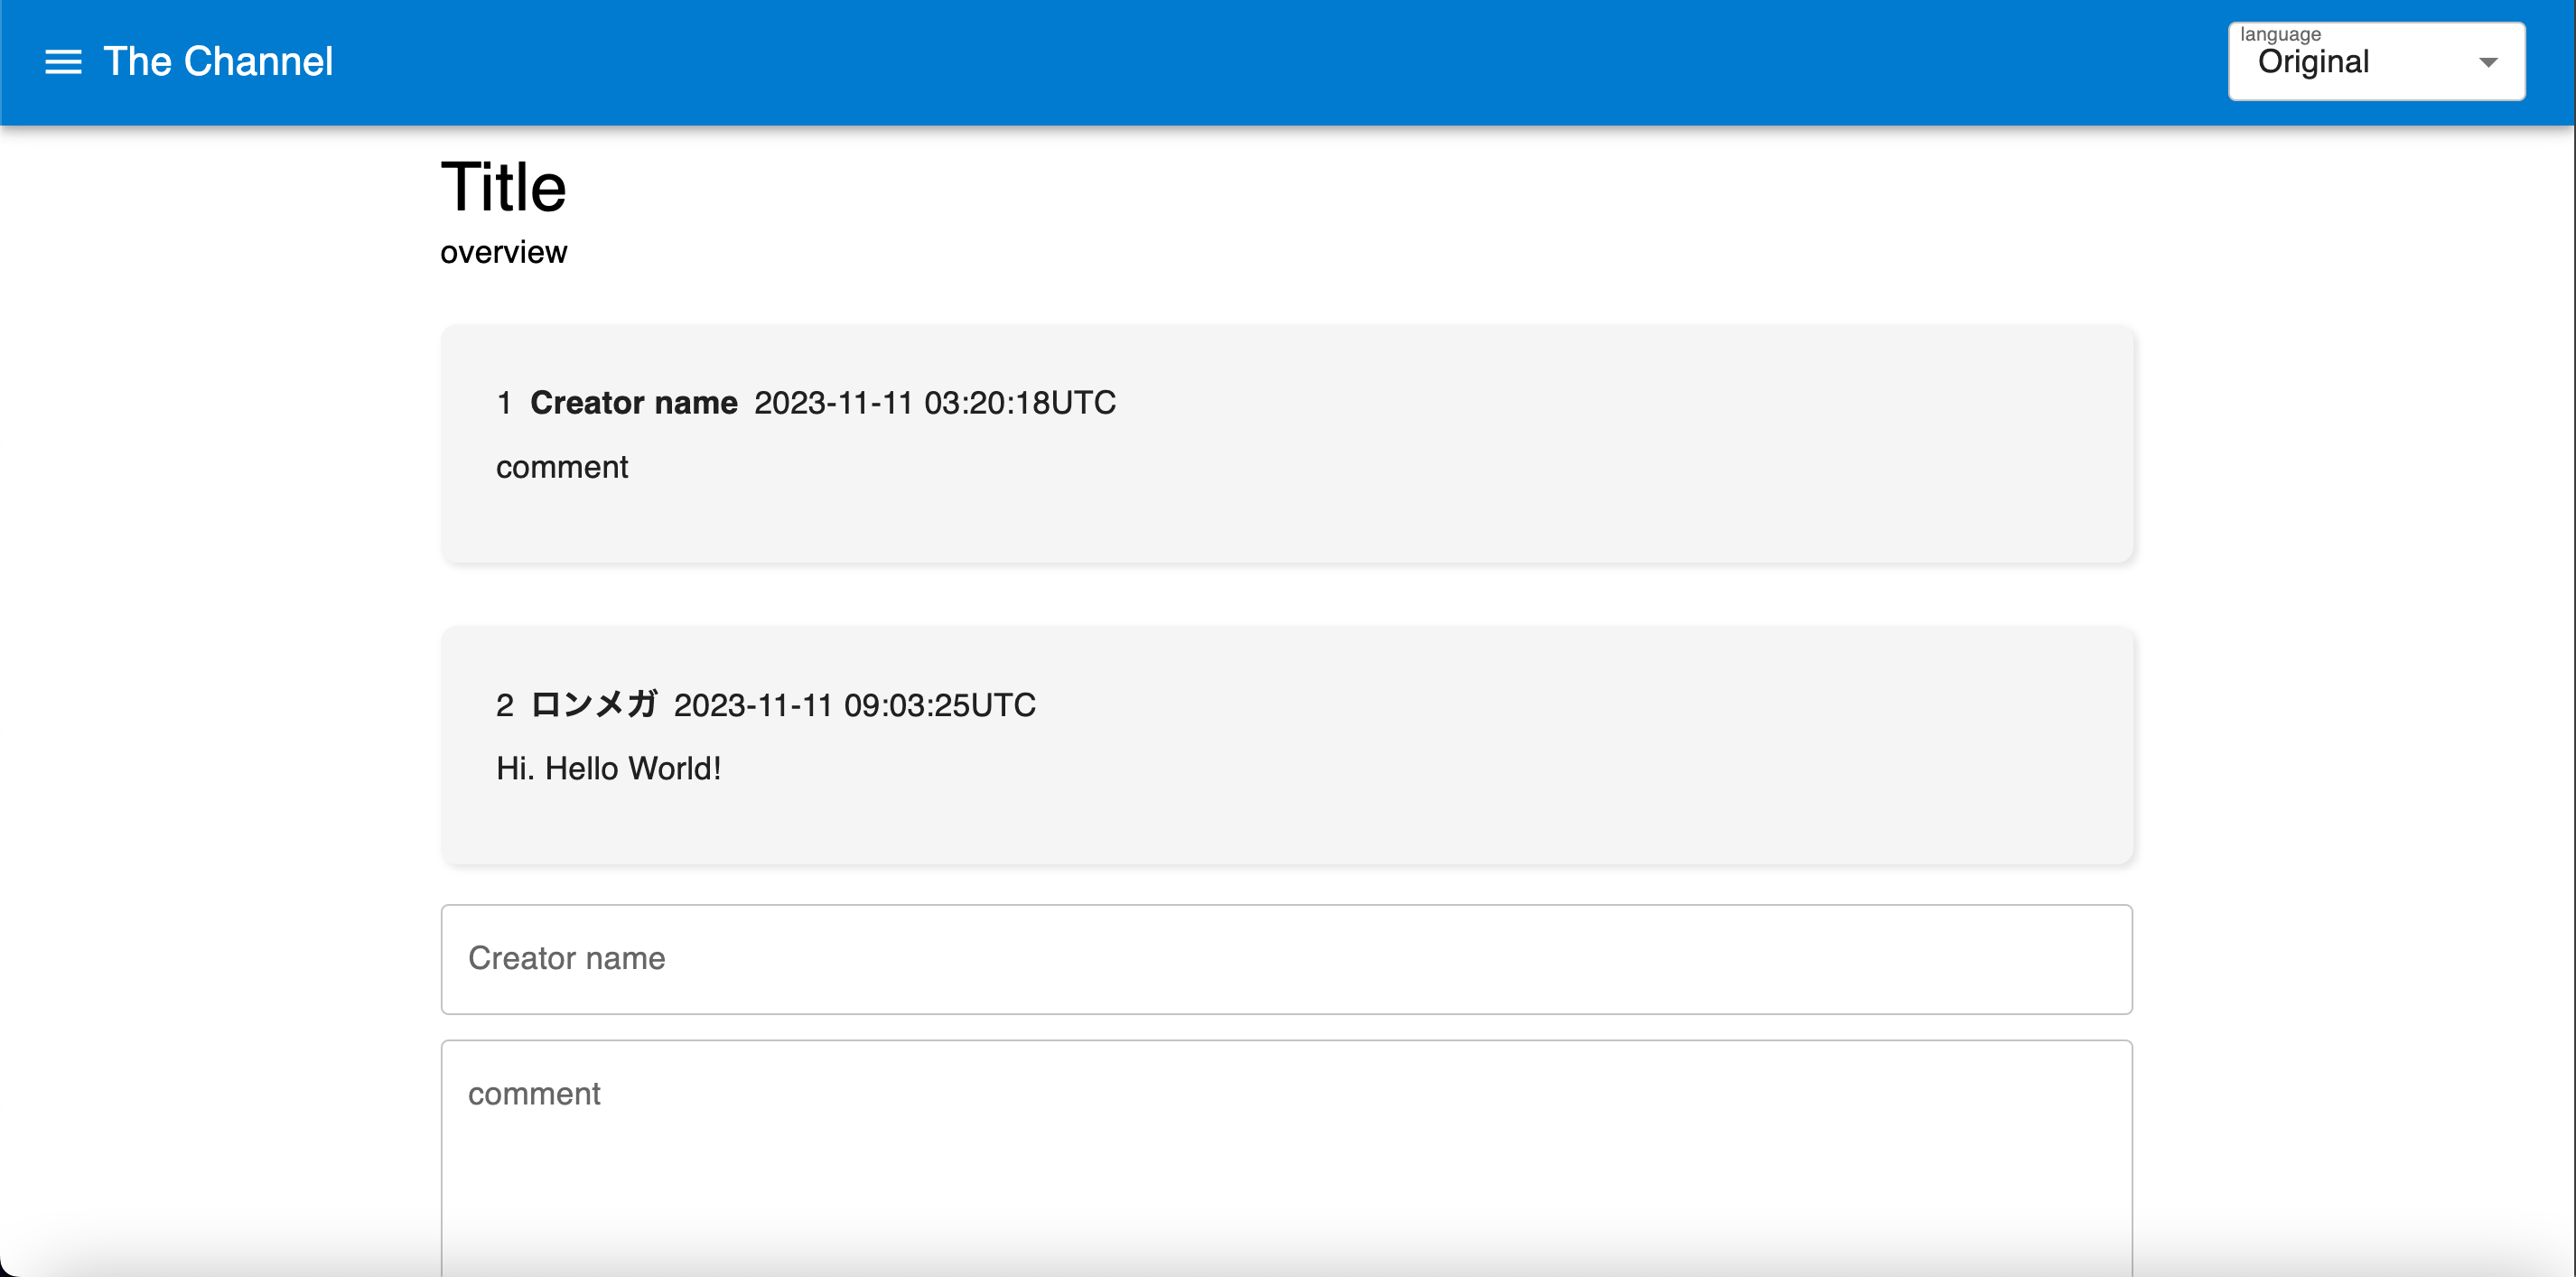
\includegraphics[width=90mm,height=45mm]{img/thread.png}

	\caption*{②スレッド詳細画面}
\end{figure}

\begin{figure}[htbp]
	\centering
	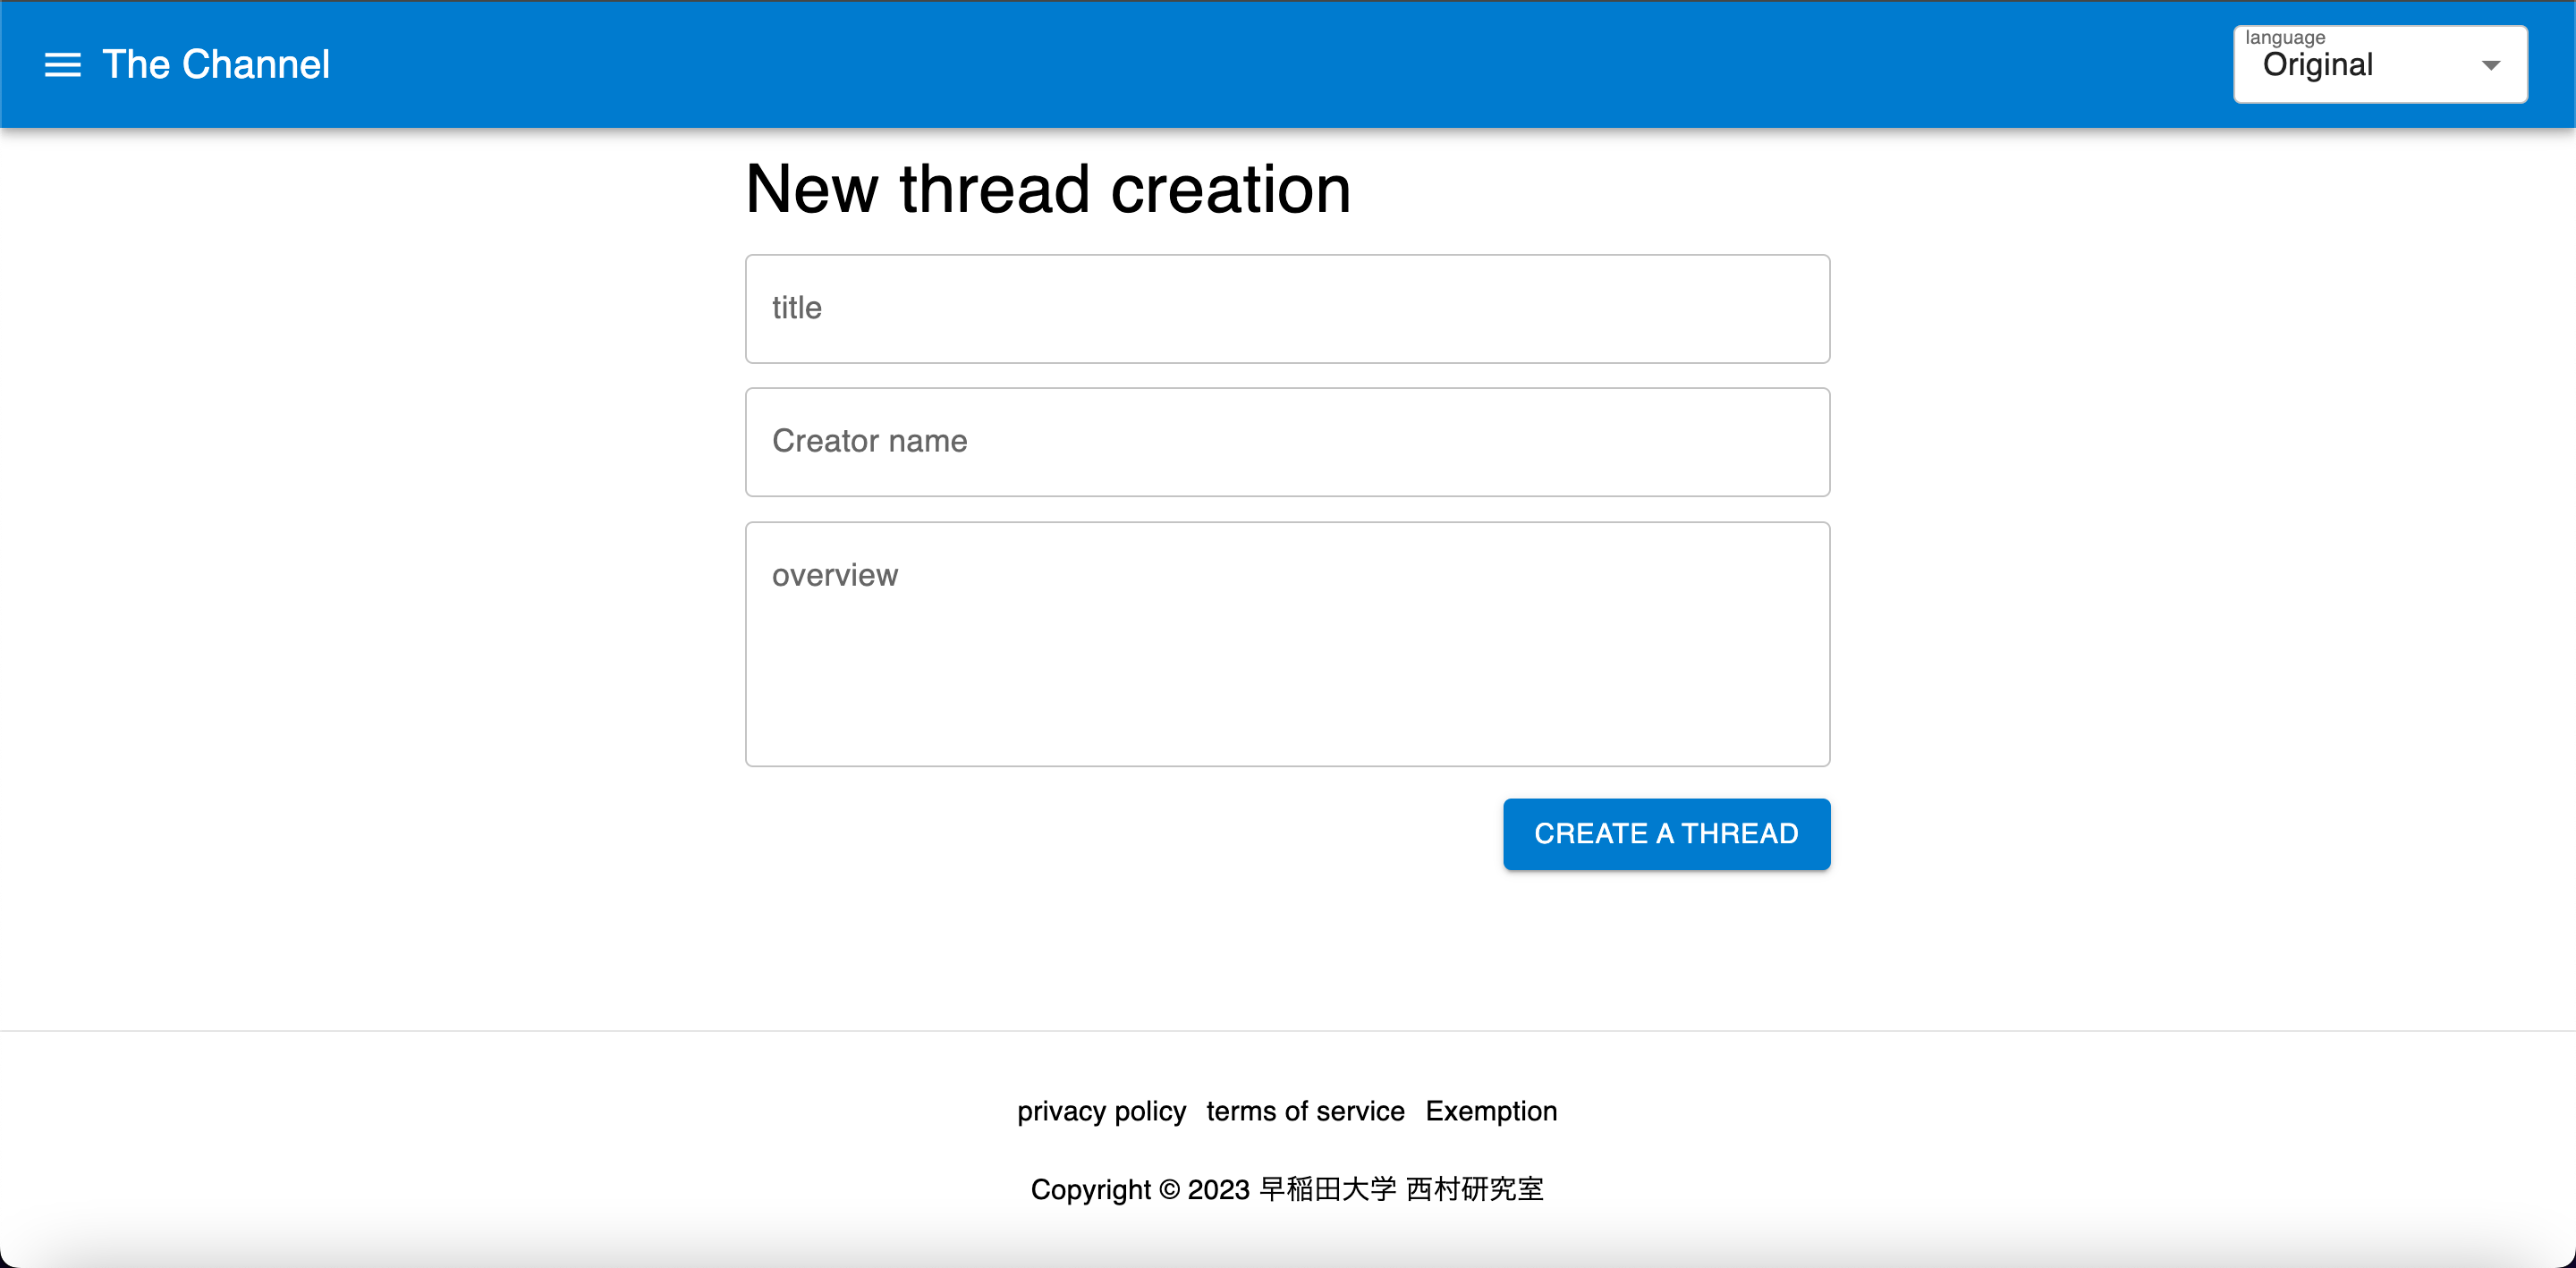
\includegraphics[width=90mm,height=45mm]{img/thread_create.png}

	\caption*{③スレッド作成画面}
\end{figure}

\begin{figure}[htbp]
	\centering
	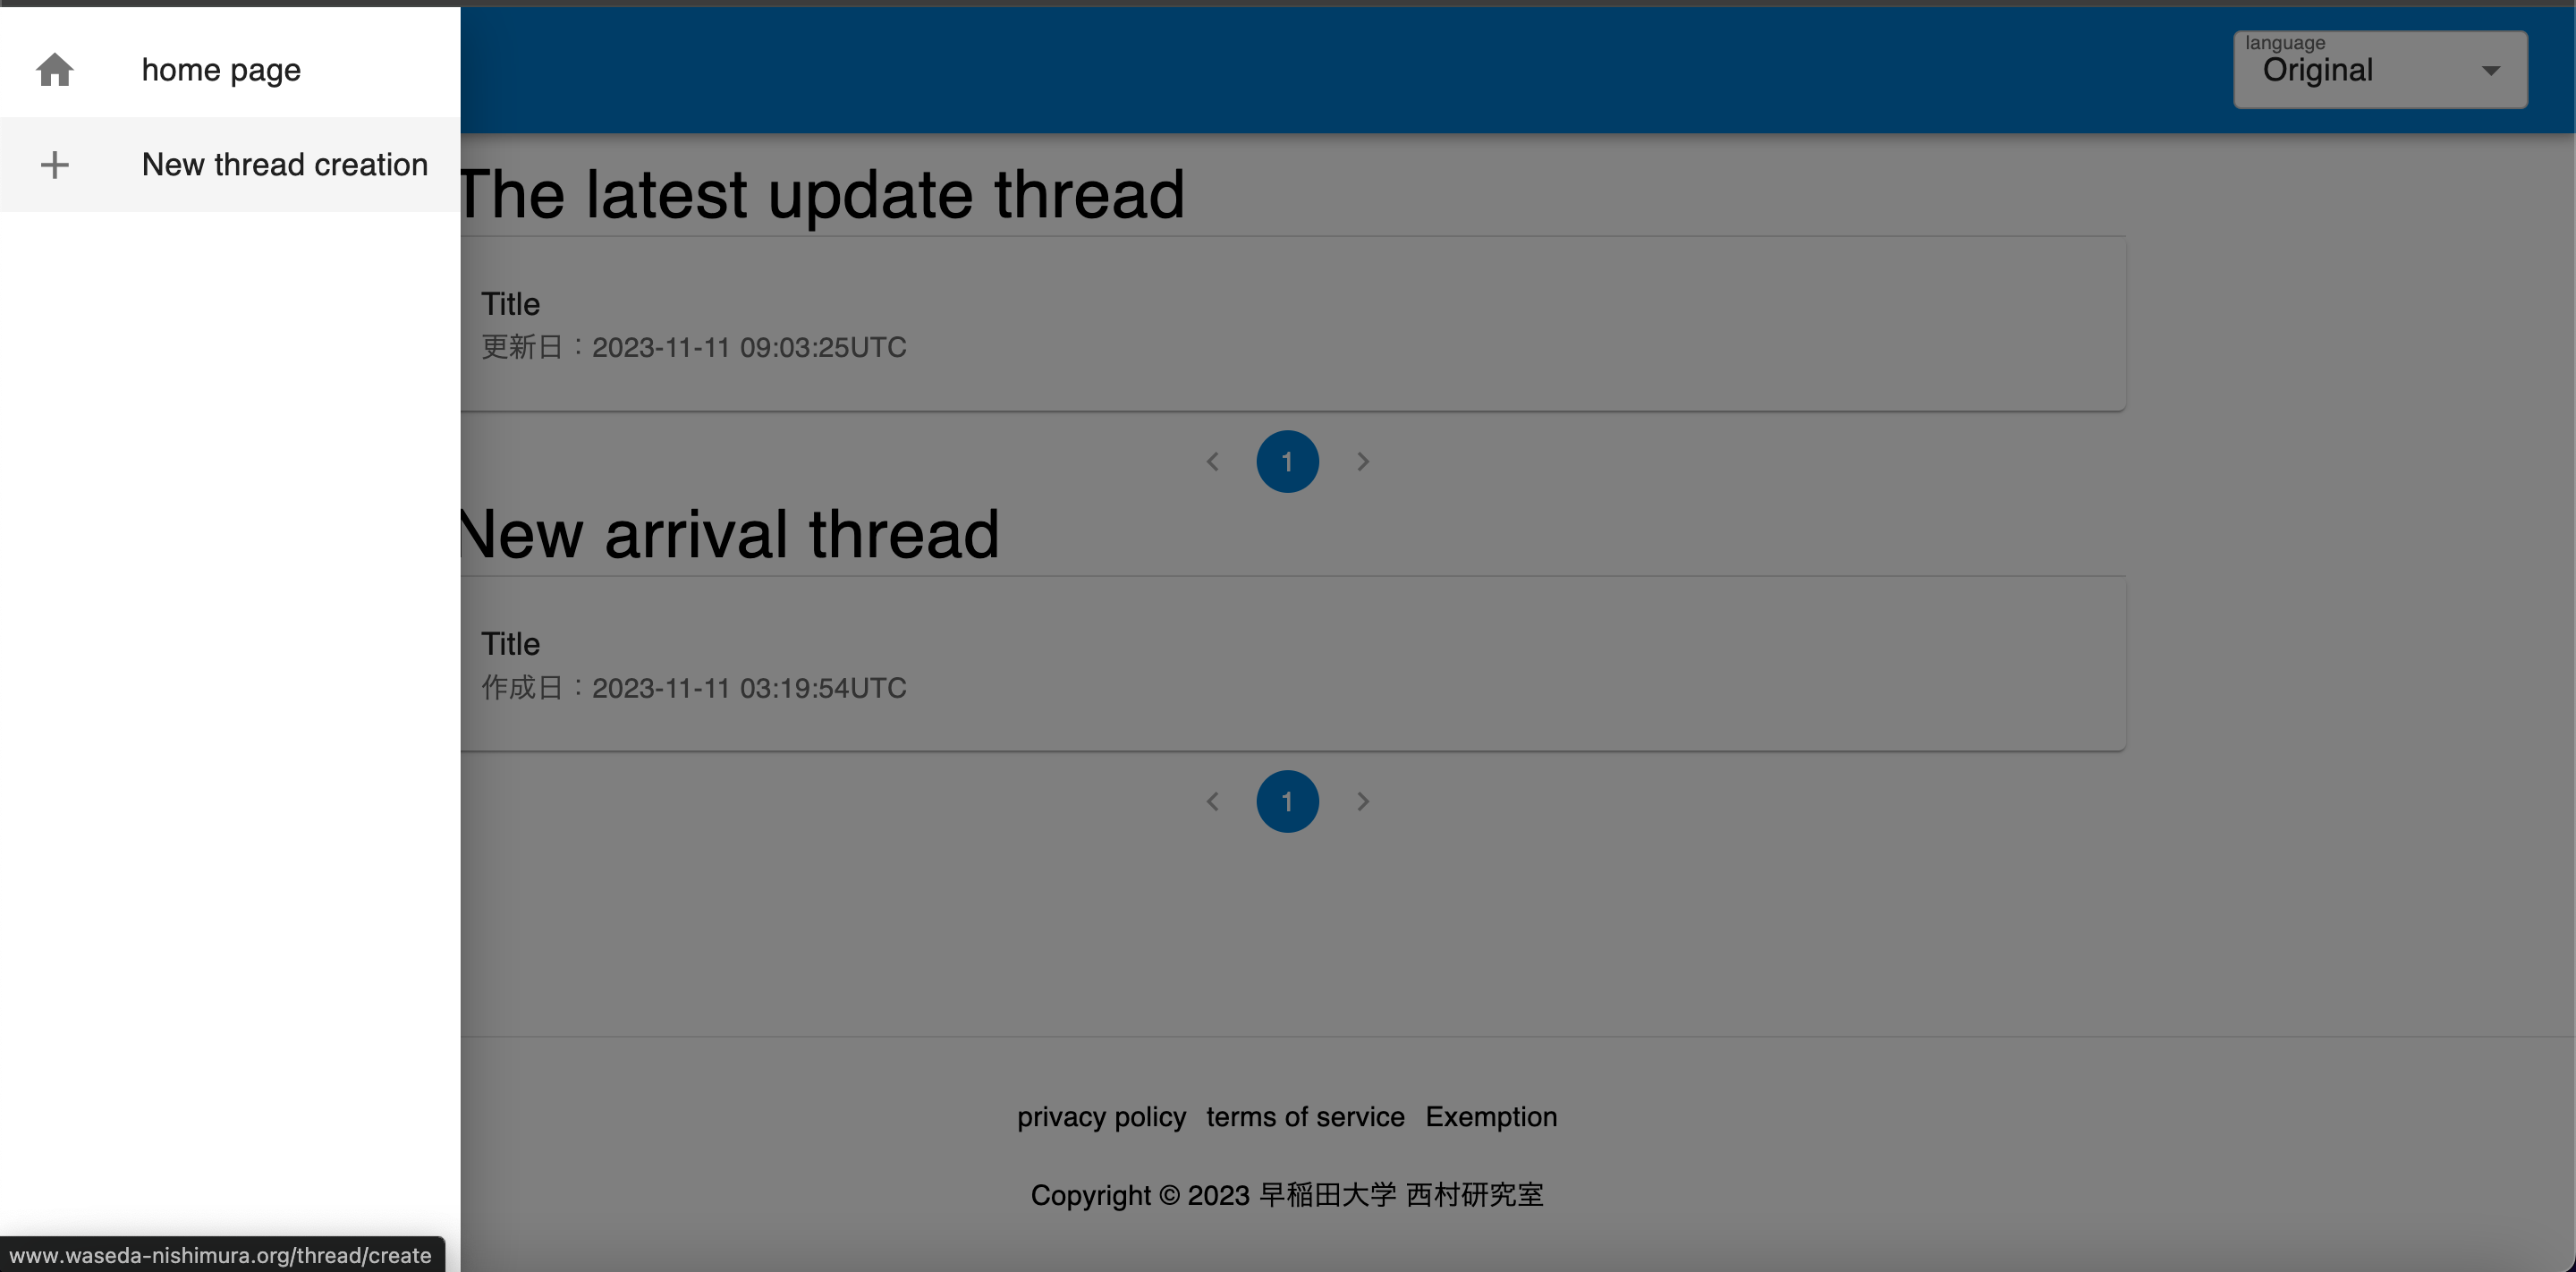
\includegraphics[width=90mm,height=45mm]{img/side_menu.png}

	\caption*{④ヘッダ表示}
\end{figure}

\begin{figure}[htbp]
	\centering
	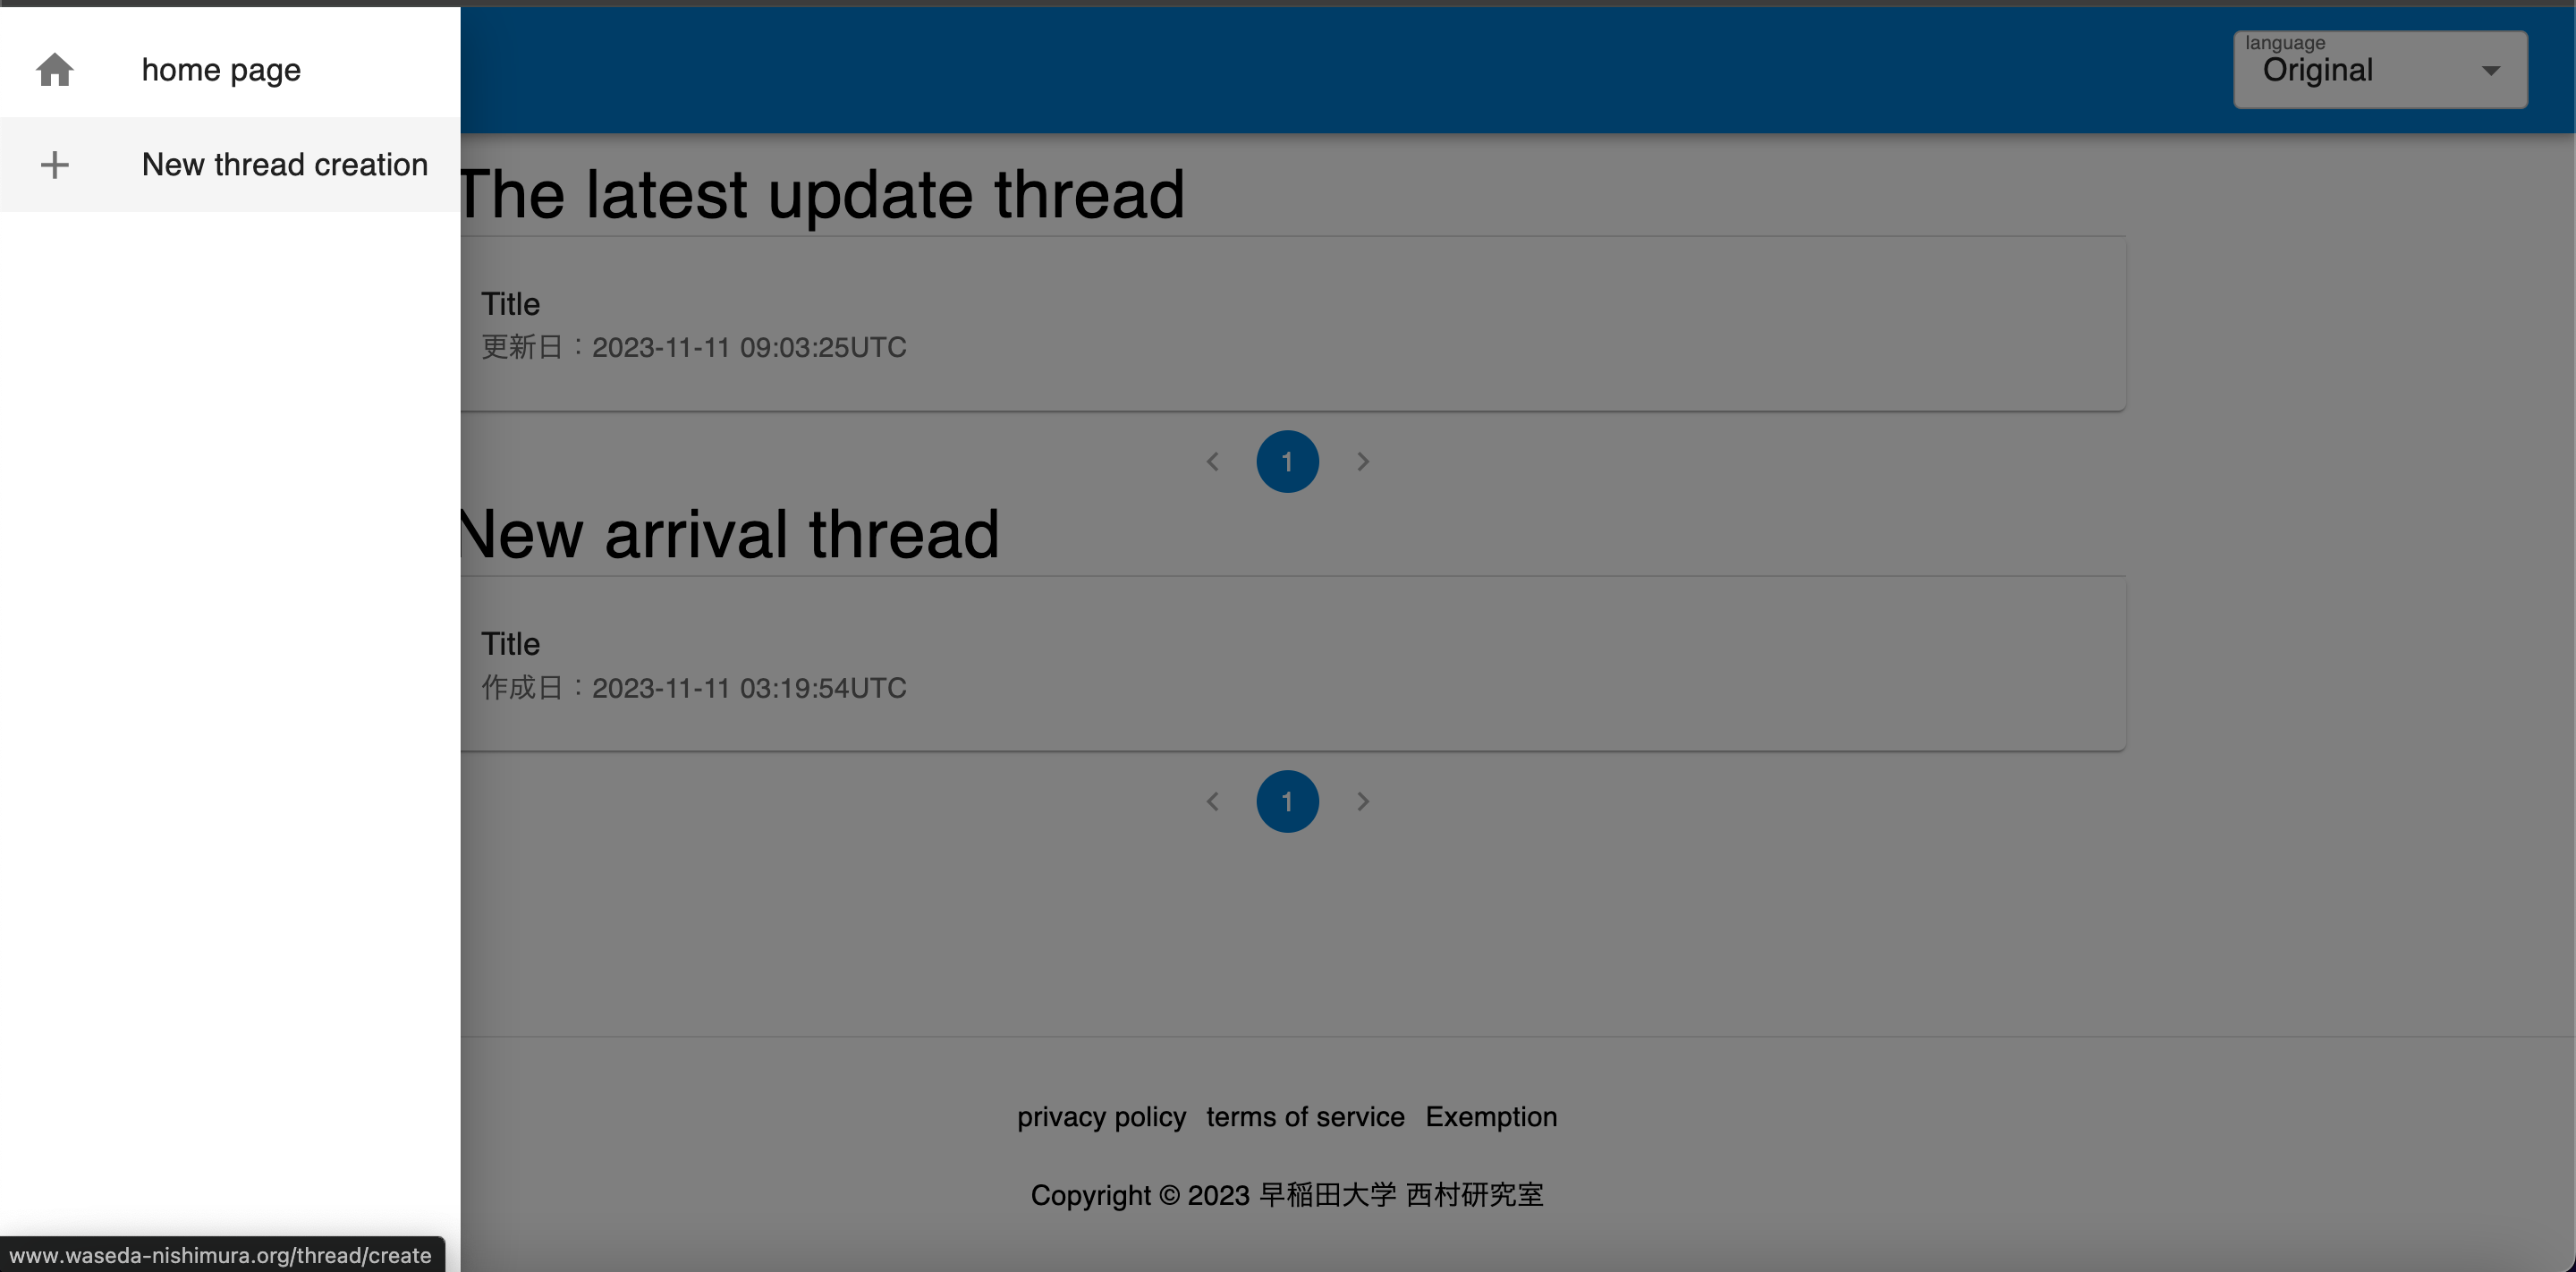
\includegraphics[width=90mm,height=45mm]{img/side_menu.png}

	\caption*{⑤サイドメニュー表示}
\end{figure}

\begin{figure}[htbp]
	\centering
	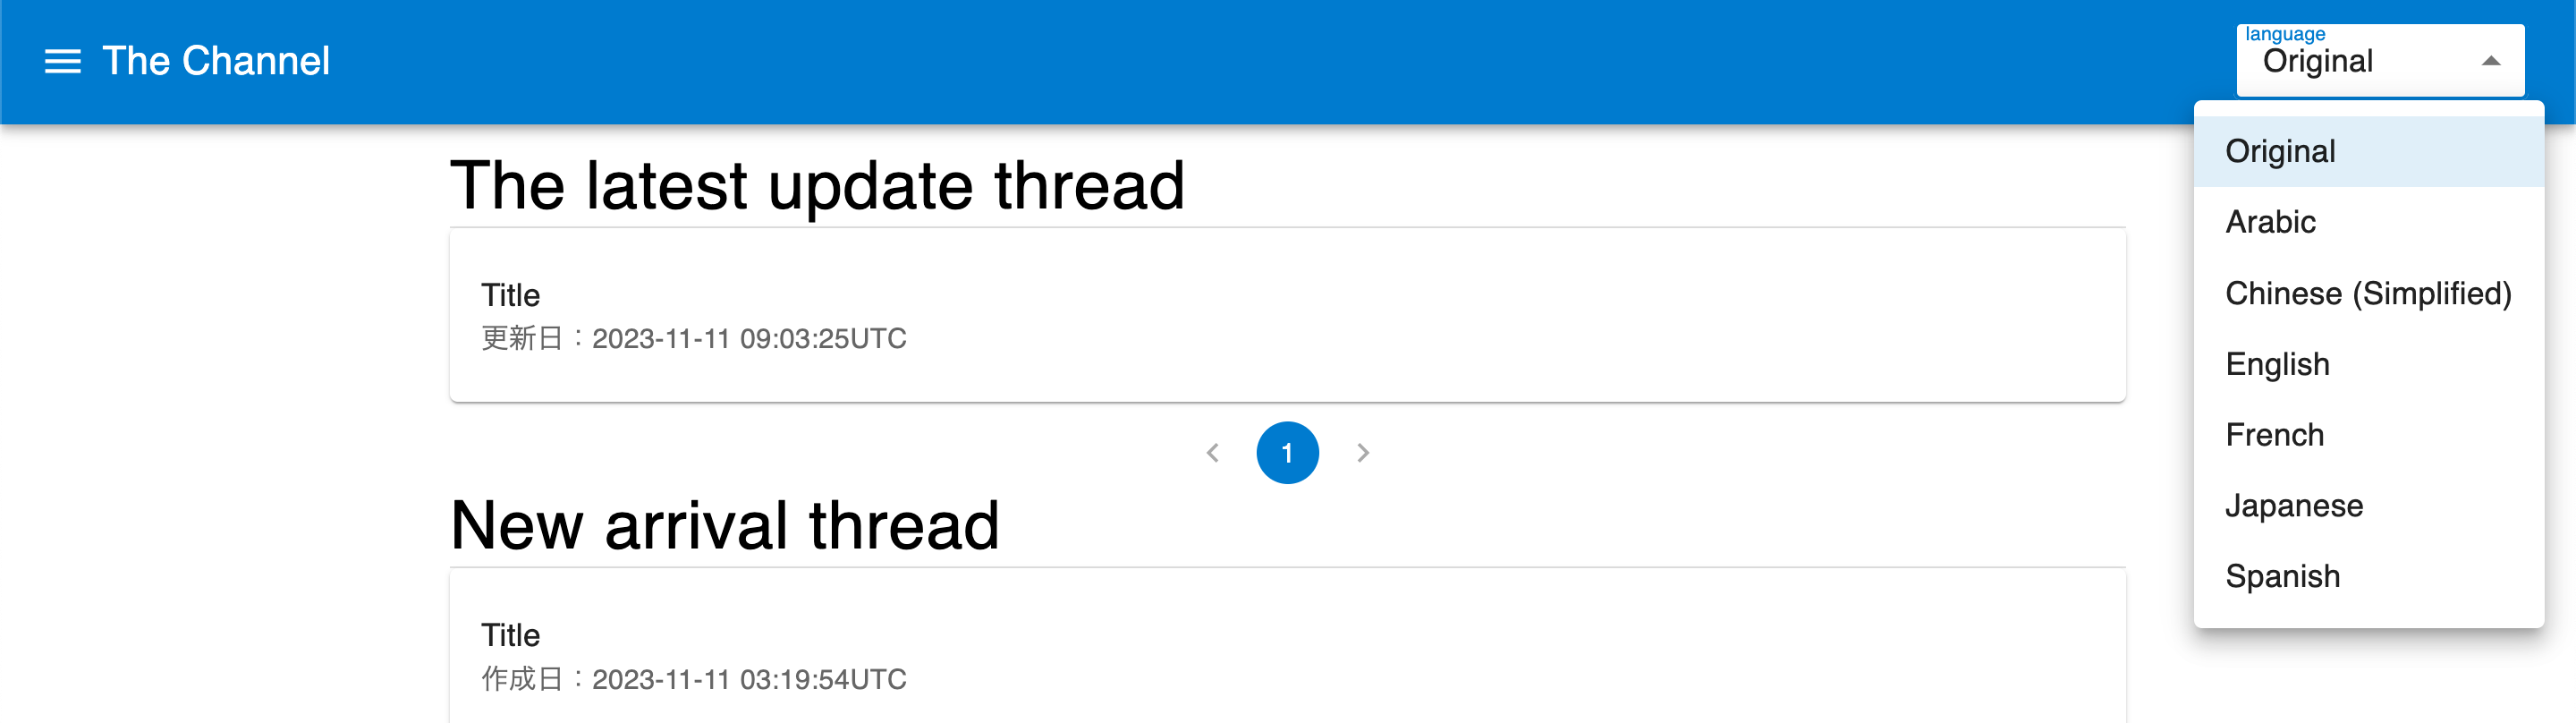
\includegraphics[width=90mm,height=45mm]{./img/select_language.png}

	\caption*{⑥言語選択表示}
\end{figure}

①トップページ画面

サイトの入り口.表示したいスレッドを選択する画面である.スレッドリストから表示したいスレッドを選択することで,詳細を表示することができる.

②スレッド詳細画面
% コメント投稿部分は分離するべきでない?
スレッドに投稿されたコメントの表示とコメントの投稿を行う画面である.表示下部のコメント投稿からコメントを投稿することができる.

③スレッド作成画面

スレッドを作成する画面である.

④ヘッダ表示

常に表示される.The Channelとの表示部分をクリックするとトップページ画面に遷移する.左部にあるメニューボタンをクリックすると⑤サイドメニューが表示される.右部にある言語選択部分をクリックすると⑥言語選択が表示される.

⑤サイドメニュー表示

トップページボタンをクリックするとトップページ画面へ,スレッド作成ボタンをクリックするとスレッド作成画面へ遷移する.サイドメニュー以外の部分をクリックするとサイドメニューは閉じられる.

⑥言語選択表示

言語を選択するとその言語に翻訳された画面へと遷移する.言語選択部分以外をクリックすると閉じられる.

⑦フッタ表示

常に表示される.プライバシーポリシー,利用規約,免責事項へのリンクがある.選択したリンクのページへと遷移する.

以下では,各機能の詳細と画面操作を説明する.

1)スレッド詳細閲覧

スレッド詳細は,トップページ画面に表示されているスレッドリストからスレッドを選択して表示する.スレッドでは,タイトル,概要が上部に表示される.
コメントはその下に連なって表示される.コメントはラベル部分とコメント部分に分かれる.ラベル部分には,コメント番号,作成者名,投稿時間が表示される.コメント部分には,投稿されているコメントが表示される.

2)スレッド作成

スレッドを作成することができる.スレッドのタイトル,作成者名,概要を入力する.全て必須項目であり,空欄があるとその旨を警告するエラーが表示され,スレッドを作成することはできない.

3)コメント投稿

スレッドに対してコメントを投稿することができる.作成者名とコメントを入力する.コメントとのみ入力必須である.作成者名が未入力であった場合は,コメントの作成者名には"NO NAME"と表示される.

4)言語選択

閲覧するための言語を選択することができる.ヘッダ右部にある言語セレクター部分をクリックすると,選択することができる言語がドロップダウンメニューとして表示される.言語をクリックすると画面が更新され,その言語に翻訳された画面に遷移する.ユーザーが選択できる言語は,日本語,英語,中国語,アラビア語,フランス語,スペイン語である.これらは,言語使用者が多い言語である.

5)スレッドリスト

ホーム画面に存在し,直近に更新があったスレッドと作成されたスレッドがそれぞれ5件ずつ表示される.5件以上のスレッドが存在する場合は,リスト下部にあるページャーを選択することで,表示されていないスレッドについても確認することができる.

6)ヘッダ

左部にあるメニューボタンをクリックするとサイドメニューを表示することができる."The Channel"と書かれている部分を選択すると,どの画面からでもトップページ画面に遷移することができる.


\begin{figure}[htbp]
	\centering
	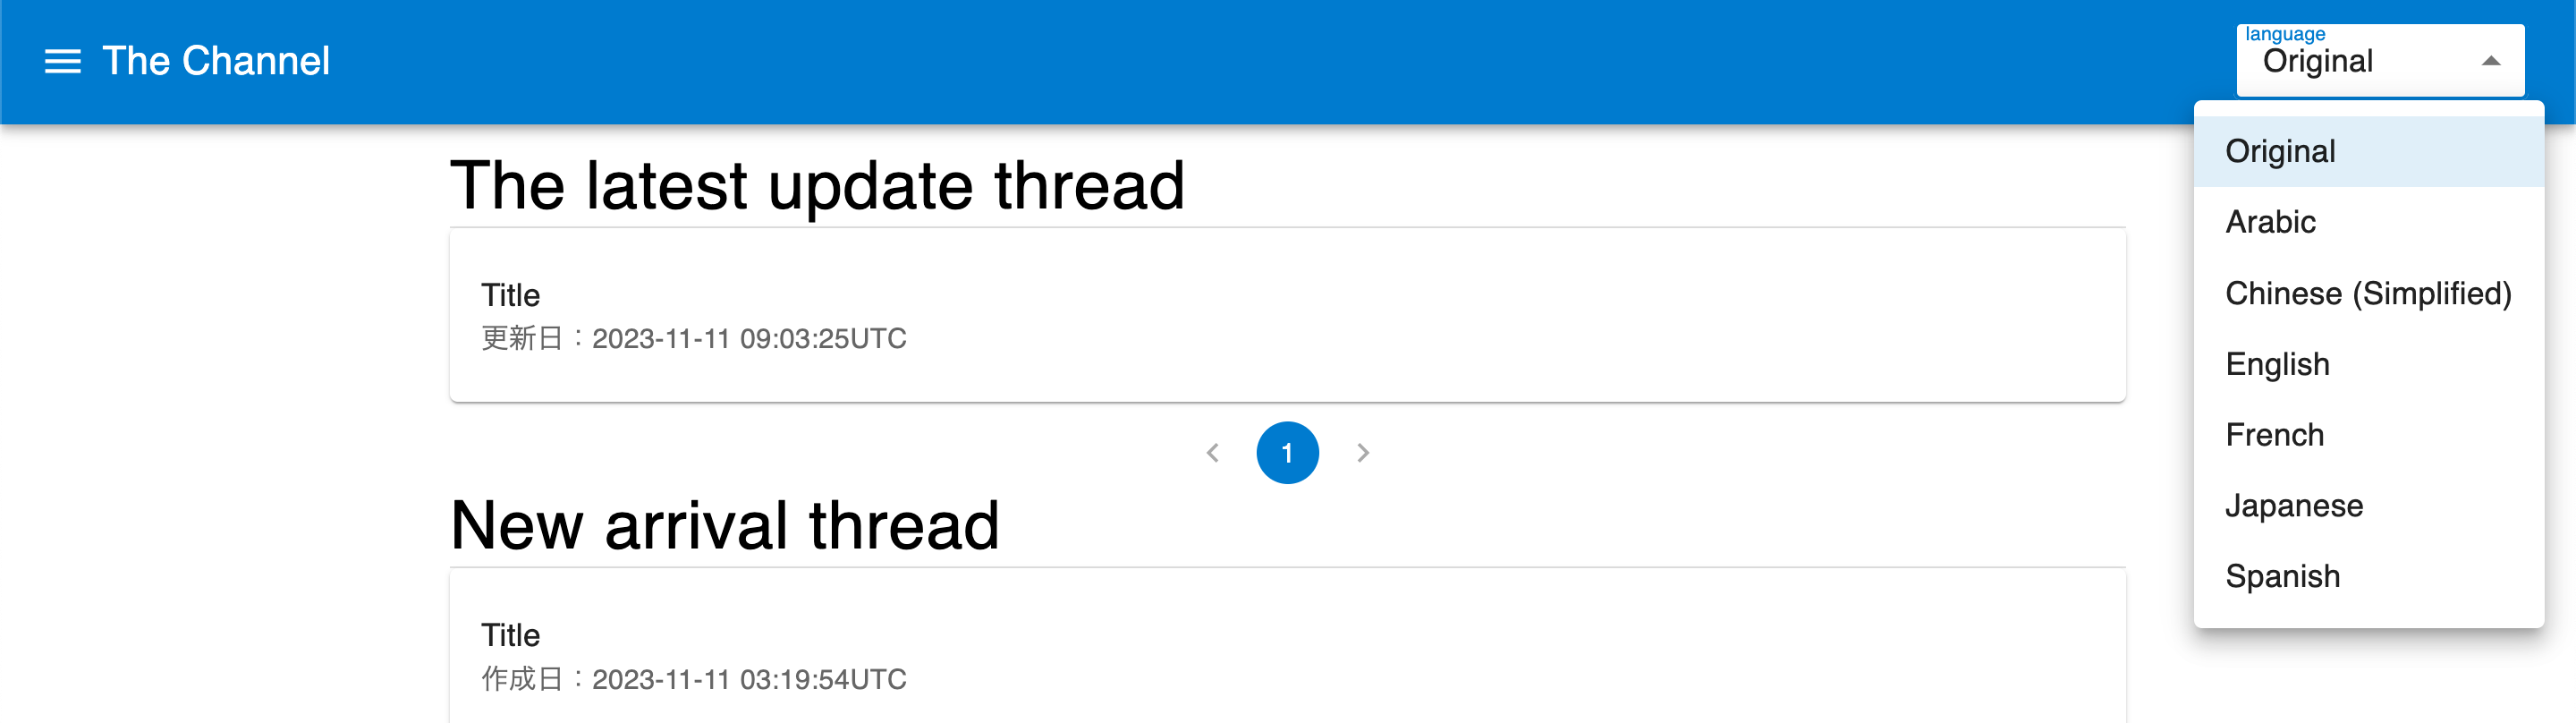
\includegraphics[width=90mm,height=45mm]{./img/select_language.png}

	\caption*{⑥言語選択表示}
\end{figure}

\begin{figure}[htbp]
	\centering
	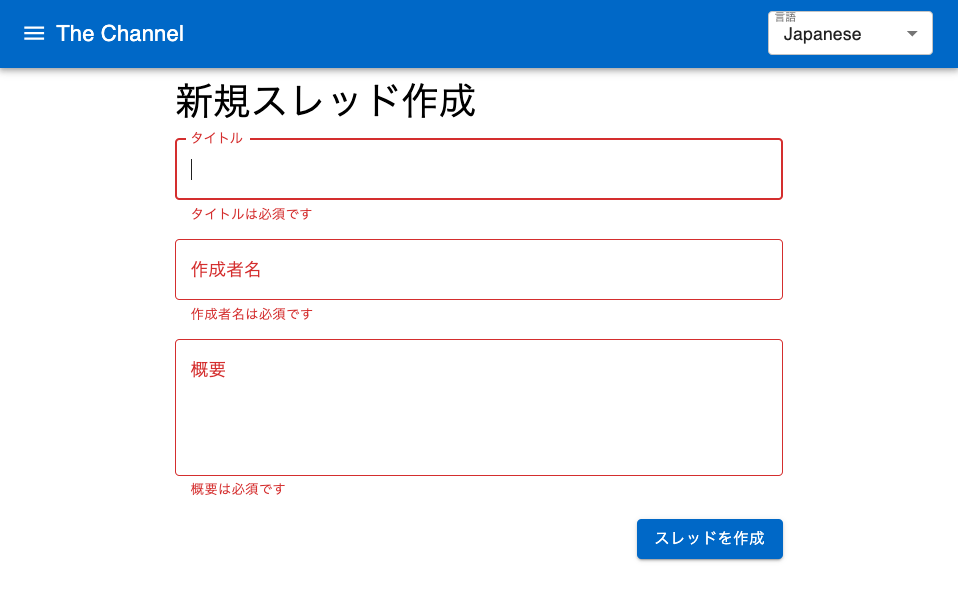
\includegraphics[width=90mm,height=45mm]{./img/thread_create_error.png}
\end{figure}

\section{システム構成の概要}
本システムは,ユーザーがWebブラウザを通じて掲示板にアクセスする構成を採用している。

% このセクションでは,システムの基本構成とその目的について概説する。

\subsection{サーバーについて}
サーバーは,さくらVPSを使用してる,オペレーティングシステムにはUbuntu 22.04.3 LTSを採用している。以下に,サーバーのCPU,ネットワークインターフェイスについての情報を記載する。

サーバーのメモリとストレージに関する情報は以下の通りである。

\subsubsection{メモリ情報}
\begin{itemize}
    \item \textbf{合計}: 7937 MB
    \item \textbf{使用中}: 1534 MB
    \item \textbf{空き}: 860 MB
    \item \textbf{バッファ/キャッシュ}: 5541 MB
    \item \textbf{利用可能}: 6094 MB
    \item \textbf{スワップ}: 0 MB
\end{itemize}

\subsubsection{ディスク使用状況}
\begin{itemize}
    \item \textbf{ファイルシステム}:
        \begin{itemize}
            \item \textbf{tmpfs}: 794 MB 使用中(1.4 MB 使用, 793 MB 空き)
            \item \textbf{/dev/vda2}: 788 GB 使用中(40 GB 使用, 708 GB 空き)
        \end{itemize}
\end{itemize}

\subsubsection{ディスク構成}
\begin{itemize}
    \item \textbf{ディスク名}: vda
    \item \textbf{サイズ}: 800 GB
    \item \textbf{タイプ}: ディスク
    \item \textbf{パーティション}:
        \begin{itemize}
            \item \textbf{vda1}: 1 MB
            \item \textbf{vda2}: 800 GB, マウントポイント: /
        \end{itemize}
\end{itemize}


サーバーのCPUに関する情報は以下のとおりである.

\begin{itemize}
    \item \textbf{アーキテクチャ}: x86\_64
    \item \textbf{CPU 操作モード}: 32-bit,64-bit
    \item \textbf{アドレスサイズ}: 46ビット物理,48ビット仮想
    \item \textbf{バイト順序}: Little Endian

    \item \textbf{CPU総数}: 6
    \item \textbf{オンラインCPUリスト}: 0-5
    \item \textbf{ベンダーID}: GenuineIntel
    \item \textbf{モデル名}: Intel Xeon Processor (Cascadelake)
    \item \textbf{CPUファミリー}: 6
    \item \textbf{モデル}: 85
    \item \textbf{コアあたりのスレッド数}: 1
    \item \textbf{ソケットあたりのコア数}: 1
    \item \textbf{ソケット数}: 6
    \item \textbf{ステッピング}: 5
    \item \textbf{BogoMIPS}: 4199.99
    \item \textbf{サポートされているフラグ}: [フラグのリスト]

    \item \textbf{ハイパーバイザのベンダー}: KVM
    \item \textbf{仮想化タイプ}: 完全仮想化

    \item \textbf{キャッシュの合計}:
        \begin{itemize}
            \item L1d: 192KiB (6インスタンス)
            \item L1i: 192KiB (6インスタンス)
            \item L2: 24MiB (6インスタンス)
        \end{itemize}

    \item \textbf{NUMAノード数}: 1
    \item \textbf{NUMAノード0 CPU}: 0-5

    \item \textbf{脆弱性と軽減策}:
        \begin{itemize}
            \item L1tf: PTE Inversionによる軽減
            \item Meltdown: PTIによる軽減
            \item Spectre v1: ユーザーコピー/swapgsバリア,ユーザーポインターのサニタイズによる軽減
            \item Spectre v2: IBRS,IBPB条件付き,STIBP無効,RSB充填,PBRSB-eIBRS Not affectedによる軽減
        \end{itemize}
\end{itemize}

サーバーのネットワークインターフェイスの設定と状態は以下の通りである.

\begin{itemize}
    \item \textbf{br-f4387cc8d030}:
    \begin{itemize}
        \item IPアドレス: 172.18.0.1/16
        \item MACアドレス: 02:42:06:18:81:07
        \item 受信パケット: 851,033 (2.0 GB)
        \item 送信パケット: 893,012 (78.0 MB)
    \end{itemize}

    \item \textbf{docker0}:
    \begin{itemize}
        \item IPアドレス: 172.17.0.1/16
        \item MACアドレス: 02:42:bf:a4:bf:64
        \item 受信パケット: 6,763 (625.9 KB)
        \item 送信パケット: 7,761 (43.2 MB)
    \end{itemize}
\end{itemize}

\subsection{セキュリティ対策}
セキュリティ対策として、ファイアウォール(UFW)とAIDS(Advanced Intrusion Detection Environment)が導入されている。設定は以下の通りである。


\begin{itemize}
    \item \textbf{状態}: アクティブ
    \item \textbf{ルール}:
    \begin{itemize}
        \item \textbf{ポート 22/tcp}: 全てのアドレスからのアクセスを許可
        \item \textbf{ポート 443/tcp}: 全てのアドレスからのアクセスを許可
        \item IPv6に関しても同様の設定
    \end{itemize}
\end{itemize}

\subsection{バックエンドについて}
バックエンドの開発においては,複数のライブラリとフレームワークが使用されている。このセクションでは,それらの技術とバージョンについて説明し,どのようにアプリケーションの機能と性能に貢献しているかを掘り下げる。ここにライブラリの詳細を書き並べる。

\subsection{フロントエンドについて}
フロントエンドの開発には,特定のライブラリとツールが利用されている。このセクションでは,これらの技術の選択とそれらがインターフェイス構築や機能開発にどのように貢献するかについて述べる。ここにライブラリの詳細を書き並べる。

\subsection{データベースについて}
データベースとしてMySQLが採用されている。このセクションでは,データベースの構成と,それがシステムにどのように統合されているかについて説明する。

\subsection{通信の取り扱いとNginxの役割}
本システムにおける通信はhttpsを通じて行われ,セキュリティを確保しつつユーザーのリクエストを効率的に処理する。ユーザーは初めにNginxを経由してフロントエンドの画面にアクセスし,画面表示に必要なデータを取得する。また,ユーザーからのPOSTアクセスはNginxを通じてバックエンドに転送され,処理される。このセクションでは,Nginxがシステム内で果たす重要な役割と,それが通信プロセスにどのように統合されているかについて詳述する。



% \section{システム構成}

% 本システムでは,ユーザーがWebブラウザを通じて掲示板にアクセスする構成を採用している.掲示板のサーバーには,さくらVPS\red{注釈的な引用的な}を使用した.

% サーバーのオペレーティングシステムは,「Ubuntu 22.04.3 LTS (コードネーム: jammy)」を使用している.

% サーバーのCPUに関する情報は以下のとおりである.

% \begin{itemize}
%     \item \textbf{アーキテクチャ}: x86\_64
%     \item \textbf{CPU 操作モード}: 32-bit,64-bit
%     \item \textbf{アドレスサイズ}: 46ビット物理,48ビット仮想
%     \item \textbf{バイト順序}: Little Endian

%     \item \textbf{CPU総数}: 6
%     \item \textbf{オンラインCPUリスト}: 0-5
%     \item \textbf{ベンダーID}: GenuineIntel
%     \item \textbf{モデル名}: Intel Xeon Processor (Cascadelake)
%     \item \textbf{CPUファミリー}: 6
%     \item \textbf{モデル}: 85
%     \item \textbf{コアあたりのスレッド数}: 1
%     \item \textbf{ソケットあたりのコア数}: 1
%     \item \textbf{ソケット数}: 6
%     \item \textbf{ステッピング}: 5
%     \item \textbf{BogoMIPS}: 4199.99
%     \item \textbf{サポートされているフラグ}: [フラグのリスト]

%     \item \textbf{ハイパーバイザのベンダー}: KVM
%     \item \textbf{仮想化タイプ}: 完全仮想化

%     \item \textbf{キャッシュの合計}:
%         \begin{itemize}
%             \item L1d: 192KiB (6インスタンス)
%             \item L1i: 192KiB (6インスタンス)
%             \item L2: 24MiB (6インスタンス)
%         \end{itemize}

%     \item \textbf{NUMAノード数}: 1
%     \item \textbf{NUMAノード0 CPU}: 0-5

%     \item \textbf{脆弱性と軽減策}:
%         \begin{itemize}
%             \item L1tf: PTE Inversionによる軽減
%             \item Meltdown: PTIによる軽減
%             \item Spectre v1: ユーザーコピー/swapgsバリア,ユーザーポインターのサニタイズによる軽減
%             \item Spectre v2: IBRS,IBPB条件付き,STIBP無効,RSB充填,PBRSB-eIBRS Not affectedによる軽減
%         \end{itemize}
% \end{itemize}

% サーバーのネットワークインターフェイスの設定と状態は以下の通りである.

% \begin{itemize}
%     \item \textbf{br-f4387cc8d030}:
%     \begin{itemize}
%         \item IPアドレス: 172.18.0.1/16
%         \item MACアドレス: 02:42:06:18:81:07
%         \item 受信パケット: 851,033 (2.0 GB)
%         \item 送信パケット: 893,012 (78.0 MB)
%     \end{itemize}

%     \item \textbf{docker0}:
%     \begin{itemize}
%         \item IPアドレス: 172.17.0.1/16
%         \item MACアドレス: 02:42:bf:a4:bf:64
%         \item 受信パケット: 6,763 (625.9 KB)
%         \item 送信パケット: 7,761 (43.2 MB)
%     \end{itemize}
% \end{itemize}

% \section{システム構成}

% 本研究で開発された多言語自動翻訳掲示板は,フロントエンドとバックエンドの開発,およびシステム環境の構築において,以下の技術を使用している.

% % \subsection{バックエンドの実装}
% % バックエンドの開発には,以下のライブラリとフレームワークが使用されている.
% % \begin{itemize}
% %     \item \textbf{FastAPI}: \texttt{fastapi==0.95.1}
% %     \item \textbf{Uvicorn}: \texttt{uvicorn==0.22.0}
% %     \item \textbf{Googletrans}: \texttt{googletrans==4.0.0rc1}
% %     \item \textbf{Pydantic}: \texttt{pydantic==1.10.7}
% %     \item \textbf{MySQL Connector}: \texttt{mysql-connector-python==8.0.33}
% %     \item \textbf{\url{httpX}: \texttt{\url{httpx==0.13.3}
% % \end{itemize}
% % これらはAPIの構築,データ処理,外部サービスとの連携に貢献している.

% \section{バックエンドの依存関係}

% バックエンドの開発において使用されたライブラリとそのバージョンは以下の通りである.

% \begin{itemize}
%     \item anyio: 3.6.2
%     \item cachetools: 5.3.1
%     \item certifi: 2022.12.7
%     \item chardet: 3.0.4
%     \item click: 8.1.3
%     \item fastapi: 0.95.1
%     \item googletrans: 4.0.0rc1
%     \item h11: 0.9.0
%     \item h2: 3.2.0
%     \item hpack: 3.0.0
%     \item hstspreload: 2023.1.1
%     \item \url{httpcore: 0.9.1
%     \item \url{httptools: 0.5.0
%     \item \url{httpx: 0.13.3
%     \item hyperframe: 5.2.0
%     \item idna: 2.10
%     \item mysql: 0.0.3
%     \item mysql-connector-python: 8.0.33
%     \item mysqlclient: 2.1.1
%     \item protobuf: 3.20.3
%     \item pydantic: 1.10.7
%     \item python-dotenv: 1.0.0
%     \item pytz: 2023.3
%     \item PyYAML: 6.0
%     \item rfc3986: 1.5.0
%     \item sniffio: 1.3.0
%     \item starlette: 0.26.1
%     \item typing\_extensions: 4.5.0
%     \item uvicorn: 0.22.0
%     \item uvloop: 0.17.0
%     \item watchfiles: 0.19.0
%     \item websockets: 11.0.2
% \end{itemize}

% これらのライブラリは,アプリケーションの様々な機能と性能に貢献しており,APIの構築,データ処理,外部サービスとの連携などに使用されている.

% % \subsection{フロントエンドの実装}
% % フロントエンドの開発には,以下のツールとライブラリが使用されている.
% % \begin{itemize}
% %     \item \textbf{React}: \texttt{react==18.2.0}
% %     \item \textbf{React-DOM}: \texttt{react-dom==18.2.0}
% %     \item \textbf{Next.js}: \texttt{next==13.3.1}
% %     \item \textbf{TypeScript}: \texttt{typescript==5.0.4}(開発依存性)
% % \end{itemize}
% % これらはユーザーインターフェースの構築,アプリケーションの構造とロジックの開発に寄与している.

% \section{フロントエンドの依存関係}

% フロントエンドの開発において使用されたライブラリとそのバージョンは以下の通りである.

% \subsection{依存関係}
% \begin{itemize}
%     \item @emotion/react: 11.11.0
%     \item @emotion/styled: 11.11.0
%     \item @mui/icons-material: 5.11.16
%     \item @mui/material: 5.13.2
%     \item @types/gtag.js: 0.0.17
%     \item @types/js-cookie: 3.0.3
%     \item @types/moment: 2.13.0
%     \item js-cookie: 3.0.5
%     \item moment: 2.29.4
%     \item moment-timezone: 0.5.43
%     \item next: 13.3.1
%     \item next-sitemap: 4.2.3
%     \item normalize.css: 8.0.1
%     \item react: 18.2.0
%     \item react-dom: 18.2.0
%     \item react-hook-form: 7.45.2
%     \item sass: 1.62.1
% \end{itemize}

% \subsection{開発用依存関係}
% \begin{itemize}
%     \item @types/node: 18.16.0
%     \item @types/react: 18.0.38
%     \item @types/react-dom: 18.0.11
%     \item @typescript-eslint/eslint-plugin: 5.59.0
%     \item @typescript-eslint/parser: 5.59.0
%     \item eslint: 8.39.0
%     \item eslint-config-next: 13.3.1
%     \item eslint-config-prettier: 8.8.0
%     \item eslint-plugin-prettier: 4.2.1
%     \item prettier: 2.8.8
%     \item typescript: 5.0.4
% \end{itemize}

% これらのライブラリは,フロントエンドのインターフェイス構築,スタイリング,機能開発に貢献しており,プロジェクトの開発とテストプロセスを支えている.

% \subsection{システム環境}
% システムの実行環境において使用されている主要なソフトウェアは以下の通りである.
% \begin{itemize}
%     \item \textbf{Nginx}: \texttt{nginx/1.25.2}
%     \item \textbf{MySQL}: \texttt{MySQL 8.0.33}
% \end{itemize}
% これらはウェブサーバーとデータベースの運用において中心的な役割を果たしている.

% 現代的なWebアプリケーション開発に適した技術スタックを用いて,柔軟かつ効率的なシステム構成を実現した.フロントエンドの開発には,TypeScript,React,Next.js,Material UI,およびSassを採用した.これらの技術選択により,ユーザーインターフェイスの高い拡張性と保守性を確保し,動的なコンテンツの迅速なレンダリングを実現している.バックエンドの開発では,PythonとFastAPIを採用し,高速な開発と性能を両立させた.データ管理には,信頼性と拡張性に優れたMySQLを使用した.そして,Nginxを用いてアクセスの受け入れとリバースプロキシを実現し,パフォーマンスの向上を図った.また,開発プロセスの効率化のためにDockerを導入した.ソースコードの管理にはGitとGitHubを使用した.

% 本掲示板の重要な役割を担っている翻訳機能については,Pythonのライブラリであるgoogletransを使用している.

\section{コンポーネント設計}

この掲示板は,表示コンポーネント,データ取得コンポーネント,データ更新コンポーネントからなる.ユーザー側インターフェイスであるWebブラウザと通信するのは表示コンポーネントである.表示コンポーネントは,画面を表示するために必要なデータをデータ取得コンポーネントに要求する.データ取得コンポーネントは,その要求を読み取り,適切に加工されたデータを表示コンポーネントに渡す.また,表示コンポーネントは,ユーザーのスレッド作成やコメント投稿に応じてデータ更新コンポーネントを呼び出し,処理を要求する.データ取得コンポーネントはその要求を読み取り,データを適切に加工して保存する.

動的な文章の翻訳はデータ取得コンポーネントで行なっている.表示コンポーネントがデータ取得コンポーネントに処理を要求する際,ユーザーが選択している言語の情報を付属させる.データ取得コンポーネントはデータを取得した後,その言語に翻訳を行い表示コンポーネントにデータを渡す.さらに,システムは翻訳の高速化と効率化のためにキャッシュ機能を実装している.一度翻訳された文章はキャッシュに保存され,同じ文章の再翻訳が必要な場合,システムはキャッシュから翻訳済みのデータを読み込む.これにより,翻訳のたびに新たに翻訳を行う必要がなくなり,システムの応答時間を大幅に短縮できる.このキャッシュシステムは,特に多言語での交流が活発な掲示板において,ユーザー体験の向上に大きく寄与している.

\section{コンポーネントの詳細}


\subsection*{表示コンポーネント}

表示コンポーネントは以下のような構成になっている.

図図図図図図図図図図図図図図図図図図図図図

ページはそれぞれ以下のファイルである.

\begin{itemize}
    \item \texttt{/pages/index.tsx} … トップページ
    \item \texttt{/pages/policy.tsx} … プライバシーポリシーページ
    \item \texttt{/pages/terms.tsx} … 利用規約ページ
    \item \texttt{/pages/404.tsx} … 404エラーページ
    \item \texttt{/pages/thread/create.tsx} … スレッド作成ページ
    \item \texttt{/pages/thread/index.tsx} … スレッドページ
\end{itemize}

表示の流れの図図図図図図図図図

図は,画面表示の際の表示コンポーネントの振る舞いをあらわしたものである.表示コンポーネントは,それぞのれページとそのページで使用される部品であるコンポーネントから成り立っている.また,画像やアイコンに関して専用のpublicフォルダを用意し,そこから読み込んでいる.

\subsection*{データ更新コンポーネント}

データ更新コンポーネントは以下のような構成になっている.

\begin{itemize}
    \item \texttt{thread\_router.py} … スレッド関連のルーティングを管理
    \item \texttt{thread\_application.py} … スレッドのアプリケーションロジックを処理
    \item \texttt{thread\_infrastructure.py} … スレッドのインフラストラクチャ関連処理
    \item \texttt{comment\_router.py} … コメント関連のルーティングを管理
    \item \texttt{comment\_application.py} … コメントのアプリケーションロジックを処理
    \item \texttt{comment\_infrastructure.py} … コメントのインフラストラクチャ関連処理
    \item \texttt{translation.py} … 翻訳機能の実装
\end{itemize}

上記のファイルリストは,以下のアーキテクチャを採用し作成された.このアーキテクチャは,明確な役割と責任を持つ複数のレイヤーに分かれている.

\paragraph{ルーターレイヤー}\mbox{}\\
\texttt{thread\_router.py} と \texttt{comment\_router.py} はルーターレイヤーに属し,外部からのリクエストを適切な処理ロジックに振り分ける役割を担う.このレイヤーは,リクエストの初期解析とルーティングを行い,システムの入口点として機能する.

\paragraph{アプリケーションロジックレイヤー}\mbox{}\\
\texttt{thread\_application.py} と \texttt{comment\_application.py} はアプリケーションロジックレイヤーを構成し、スレッドとコメントに関するビジネスロジックを実装する。このレイヤーは、アプリケーションの核心的な機能を担い、データの処理やビジネスルールの適用を行う。

\paragraph{インフラストラクチャレイヤー}\mbox{}\\
\texttt{thread\_infrastructure.py} と \texttt{comment\_infrastructure.py} はインフラストラクチャレイヤーに属し,データベースとのやり取りやデータの永続化を管理する.このレイヤーは,システムのデータ層に関わる処理を担当し,データの整合性と安全性を保証する.

\paragraph{翻訳機能}\mbox{}\\
\texttt{translation.py} は,これらのレイヤーとは別に,システム全体の翻訳機能を提供する.このファイルは,多言語サポートを実現し,異なる言語間でのコミュニケーションを可能にする.

以上のように,各レイヤーは特定の役割を持ち,システム全体の効率的かつ整理された運用を支援する.このレイヤー化されたアーキテクチャにより,システムの拡張性,保守性,およびスケーラビリティが向上している.


\section{データ設計}

\subsection*{Threadsテーブル}

スレッドの情報を格納するテーブルである.

\begin{adjustbox}{width=\textwidth,center}
	\begin{tabular}{lll}
	\toprule
	\textbf{カラム名} & \textbf{データ型} & \textbf{説明} \\
	\midrule
	ThreadID   & INT PRIMARY KEY AUTO\_INCREMENT & スレッドのID \\
	Title      & VARCHAR(255) & スレッドのタイトル \\
	CreatedAt  & TIMESTAMP & 作成日時 \\
	UpdatedAt  & TIMESTAMP & 更新日時 \\
	UserName   & VARCHAR(255) & ユーザー名 \\
	Content    & LONGTEXT & 内容 \\
	Language   & VARCHAR(8) & 言語 \\
	\bottomrule
	\end{tabular}
\end{adjustbox}

\subsection*{Commentsテーブル}

スレッドに投稿されたコメントを格納するテーブルである.

\begin{adjustbox}{width=\textwidth,center}
	\begin{tabular}{lll}
	\toprule
	\textbf{カラム名} & \textbf{データ型} & \textbf{説明} \\
	\midrule
	CommentID  & INT PRIMARY KEY AUTO\_INCREMENT & コメントID \\
	ThreadID   & INT & スレッドID \\
	UserName   & VARCHAR(255) & ユーザー名 \\
	Content    & TEXT & コメント内容 \\
	CreatedAt  & TIMESTAMP & 作成日時 \\
	Language   & VARCHAR(8) & 言語 \\
	\bottomrule
	\end{tabular}
\end{adjustbox}

\subsection*{Cookie}

Cookieを使用してユーザーの言語選択を記録し,その設定に基づいてユーザーに表示する際に翻訳を行う.この機能により,ユーザーは毎回言語を選択する必要がなく,効率的かつ快適にアプリを利用できる.

\begin{adjustbox}{width=\textwidth,center}
    \begin{tabular}{ll}
    \toprule
    \textbf{Cookieの名称} & \textbf{内容} \\
    \midrule
    SelectedLanguage & ユーザーが選択した言語設定 \\
    \bottomrule
    \end{tabular}
\end{adjustbox}

Cookie「SelectedLanguage」は,ユーザーが最後に選択した言語を記録するものである.この情報は次回のウェブサイト訪問時に参照され,ユーザーが以前に選択した言語でインターフェースが表示されるようになる.この機能はユーザビリティを向上させ,多言語対応の効率を高める.


\chapter{利活用についての分析}

本研究で開発された多言語自動翻訳掲示板システムの利活用について分析するためには,ユーザーに使用してもらうことが必要である.このシステムは,異なる文化や言語背景を持つユーザーが交流し,情報を共有するためのプラットフォームとして機能することを目的としている.従って,多様なユーザーグループを獲得し,継続的に参加を促すことは,システムの成功にとって非常に重要である.

システムの普及に際して,ソーシャルメディアは重要な役割を担う.本研究では,Twitterを用いてシステムの普及を図った.Twitterは広範なユーザーネットワークを有し,迅速な情報伝播が可能であるため,新しいテクノロジーの告知に適したプラットフォームである.このアプローチにより,ターゲットオーディエンスに直接アピールし,関心を引きつけることが期待される.

\begin{thebibliography}{99}

\bibitem{omukai2006} 
大向一輝 (2006). SNSの現在と展望-コミュニケーションツールから情報流通の基盤へ-. 情報処理,47(9): 993-1000.

\bibitem{ogawa2009} 
小川泰弘,福田ムフタル,外山勝彦 (2009). 日本語ーウイグル語翻訳掲示板システム. 言語処理学会 第15回年次大会発表論文集,15: 212-215.

\bibitem{kageura2017} 
影浦峡 (2017). 改めて,翻訳とは何か:Google NMTが使える時代に. 言語処理学会 第23回年次大会発表論文集,23: 931-934.

\bibitem{kameda2022} 
亀田倫史 (2022). 機械学習とバイオテクノロジー. 生物工学会誌,100(11): 588.

\bibitem{nakazawa2017} 
中澤敏明 (2017). 機械翻訳の新しいパラダイム:ニューラル機械翻訳の原理. 情報管理,60(5): 299-306.

\bibitem{notsu2009} 
野津誠 (2009). 日韓翻訳掲示板「enjoy Korea」終了へ,理由は利用率の低下. 株式会社インプレス,\url{https://internet.watch.impress.co.jp/cda/news/2009/02/12/22405.html}(参照日2023.07.17)

\bibitem{fujii2005} 
藤井薫和,重信智宏,吉野孝 (2005). 異文化間コミュニケーションのための機械翻訳を用いたチャットシステムAnnoChatの開発と適用. 情報科学技術フォーラム一般講演論文集,4(3): 437-438.

\bibitem{funakoshi2004} 
船越要,藤代祥之,野村早恵子,石田料亨 (2004). 機械翻訳を用いた協調作業支援ツールへの要求条件—日中韓馬異文化コラボレーション実験からの知見. 情報処理学会論文誌,45(1): 112-120.

% \bibitem{miyabe2009} 
% 宮部真衣,吉野孝 (2009). 折り返し翻訳を用いた翻訳リペアのチャットコミュニケーションへの影響.

\bibitem{miyabe2010} 
宮部真衣,吉野孝 (2010). 機械翻訳を介したチャットコミュニケーションにおける精度判定に基づく送信拒否の適用可能性. 情報処理学会論文誌,51(3): 784-795.

\bibitem{muramoto2022} 
村本麻衣 (2022). 自動翻訳機能からの自立:学習者による気づきを通じて. ドイツ語教育 = Deutschunterricht in Japan / 日本独文学会ドイツ語教育部会 編,26: 119-125.

\bibitem{yoshino2006} 
吉野孝,藤井薫和,重信智宏 (2006). 異文化間コミュニケーションのためのカスタマイズ可能なユーザインタフェイスを持つチャットシステムCustomChatの開発. 情報処理学会研究報告 = IPSJ SIG technical reports,(60): 13-18.

\bibitem{deepl} 
DeepL (2023). DeepL. \url{https://jobs.deepl.com/}(参照日2023.07.08)

\bibitem{googlecloud} 
Google Cloud (2023). Translation AI. \url{https://cloud.google.com/translate?hl=ja}(参照日2023.07.17)

\bibitem{loki} 
Loki Technology,Inc (2023). 5ちゃんねる. \url{https://5ch.net/}(参照日2023.07.17)

\bibitem{googletrans} 
PyPI (2023a). googletrans 3.0.0. \url{https://pypi.org/project/googletrans/}(参照日2023.07.17)

\bibitem{deeplpy} 
PyPI (2023b). deepl 1.15.0. \url{https://pypi.org/project/deepl/}(参照日2023.07.17)

\bibitem{reddit} 
Reddit Inc (2023). reddit. \url{https://www.redditinc.com/}(参照日2023.07.08)

\bibitem{server_world}
Server World (2022). AIDE : ホスト型 IDS. \url{https://www.server-world.info/query?os=Ubuntu_22.04&p=aide}(参照日2023.12.2)

\end{thebibliography}
    
% \begin{thebibliography}{99}
% % \bibitem{rika} 国立天文台編,理科年表 (丸善)
% % \bibitem{ten} 天文年鑑,誠文堂新光社.
% \end{thebibliography}

\end{document}
